\subsection{Broker}\label{sec:impl-broker}

The broker sub-system of our city simulator is written in Elixir, and leverages
Wabbit (a GenStage and RabbitMQ adapter).

A broker is basically a pipeline through which messages are processed:

\begin{itemize}
  \item a \texttt{BackendControlListener} process listens the RabbitMQ shared
    with the middleware nodes, waiting for control messages
  \item a \texttt{Daemon} process listens the RabbitMQ shared with the
    middleware nodes, waiting for application-logic related messages
  \item a \texttt{ContentEnricher} process 
  \item a \texttt{Forwarder} process puts messages on output queues of a
    RabbitMQ broker shared with the application server
\end{itemize}

A visual representation of this can be found in Figure \ref{fig:broker-arch}.

\begin{figure}[H]
  \centering
  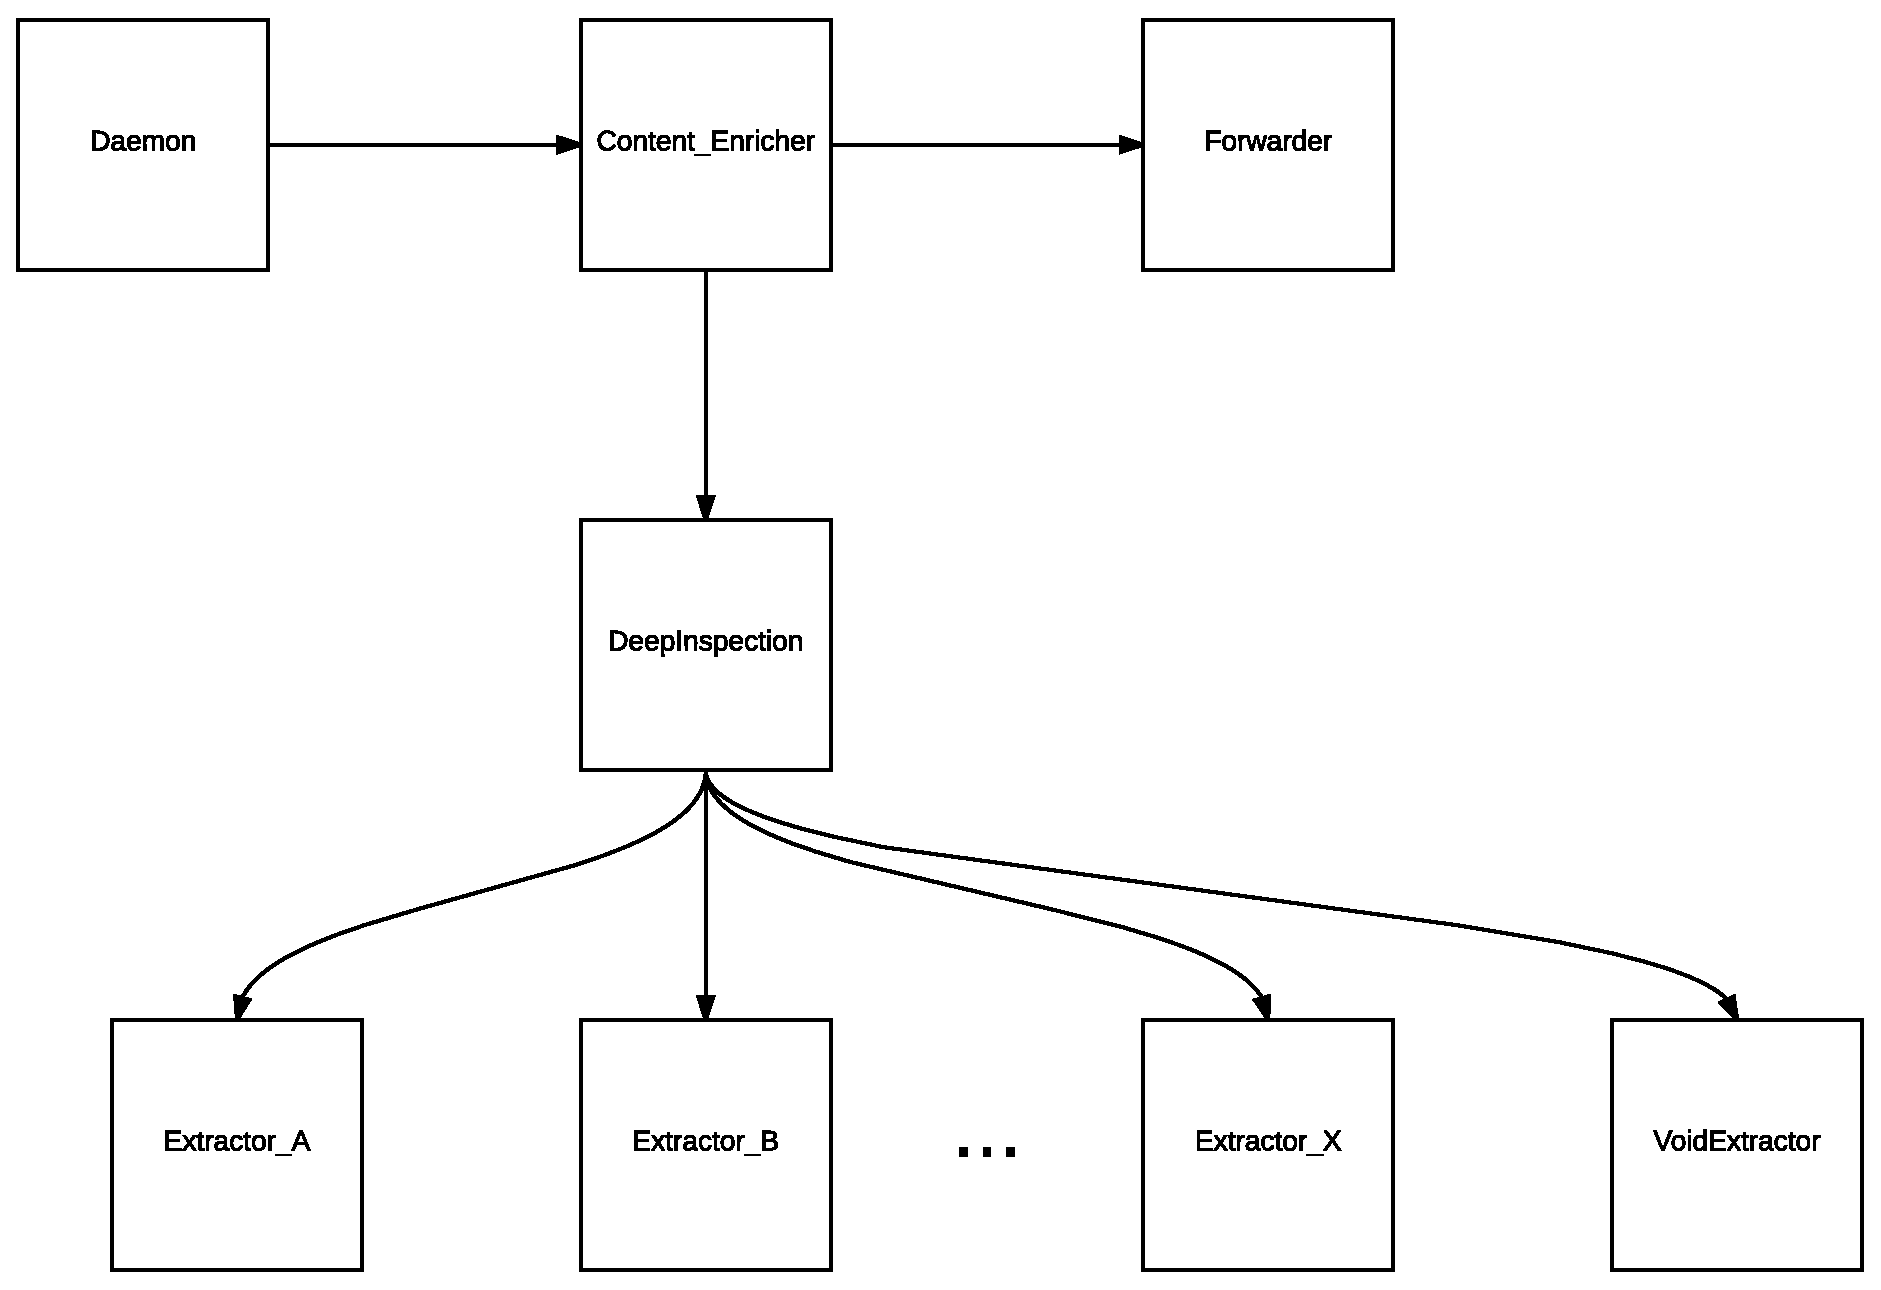
\includegraphics[width=\columnwidth]{images/implementation/broker.eps}
  \caption{Broker architecture}
  \label{fig:broker-arch}
\end{figure}

Clearly, each one of these processes could be arbitrarily replicated, for
instance we may decide to have 5 \texttt{BackendControlListener}s, 3
\texttt{Daemon}s, 6 \texttt{ContentEnricher}s and 8 \texttt{Forwarder}s, and
all of this would be fairly trivial to implement.

On the other hand, one could also think to spawn multiple copies of these
processes for being able to cope with increased load.
This might be done by evaluating the processes' demand and offer variables,
choosing some thresholds and spawning other supervised workers on demand.

Each \texttt{ContentEnricher} transforms messages thanks to a
\texttt{DeepInspection} module, which indeed opens up the message and looks
inside to extract information.
It does so with the help of a series of Extractors modules\footnote{we did not
defined an Elixir Protocol, i.e., intereface for them but it would have been
quite easy} which actuate the process. There is also a \texttt{VoidExtractor}
module, which basically is a fallback case for an unidentified request.

\paragraph{Communication from frontend to backend}
Actually, our broker provides a means of communication from the frontend to
the backend as well.
We made this implementation choice because, even if it involves a flow of
information which goes in the opposite direction as the aforementioned
pipeline, we would have to instantiate another microservice to manage the
communication from the frontend to the backend.
Nevertheless, since at the moment the frontend contacts the backend only for
requiring a boot, we thought it was not meaningful to have a full-blown
microservice just for sending one control message, and we embodied
bi-directional communication into our broker.

\paragraph{Achieving transparency}
In order to have a glimpse of the reason why we say the application is
transparent to the middleware and viceversa, here we will make an example which
involves the broker subsystem.

When travellers manage to tread a new piece of infrastructure, they publish an
event by issuing an asynchronous request to the middleware. However, they do it
without knowing (or specifying) if the tread operation was local or remote,
because (despite the qualified name of the Callbacks package) travellers just
state a Tread operation was completed.
For what concers the middleware, it sees an asynchronous request named
``TREAD''. Since the middleware does not know anything about the application
logic domain, it just recognizes an asynchronous event was issued by the
application layer and forwards the message to our broker.
The broker subsystem is instead able to distinguish if a movement was local or
remote by means of a little hack:

\begin{itemize}
  \item the application layer states the operation involves a treadable entity,
    and it refers to it by its logical identifier
  \item upon the message reception, the middleware looks up for the recipient
    node by performing name resolution on the identifier specified in the
    message headers
  \item the middleware then appends the recipient and sender fields to the
    (middleware-layer) message, which gets forwarded to the broker. We do not
    lose transparency, since the recipient and sender fields carry information
    about the backend nodes involved in the operation;
  \item if the broker reads two different values for the sender and the
    recipient fields, then it knows this is a remote operation, whilst in the
    case the sender and the recipient fields are equal it knows a traveller did
    not move to another district.
\end{itemize}
